% \section{The reciprocal theorem and equaitons for a droplet force and Stresslet}
% \label{ap:reciprocal}




\section{Governing equations and solutions}


At the leading order in droplet volume fraction, the closure problem is equivalent to that of an isolated droplet in an infinite medium \citet{hinch1977averaged}. 
Hence, we consider the problem of an isolated test droplet immersed in an arbitrary quadratic flow without the presence of fluid inertia. 
The disturbances pressure and velocity field relative to the position of a test droplet are noted $\textbf{u}_{o}$, $\textbf{u}_{i}$, $p_{o}$ and $p_{i}$, for the velocity outside the test droplet, the velocity inside the droplet, the pressure outside the droplet and the pressure inside the droplet, respectively. 
The corresponding ``undisturbed field'' or ensemble averaged (unconditionally) are $\textbf{u}_f$ and $p_f$, because we compute the disturbance fields relative to the continuous phase quantities. 

On \ref{fig:disturbance} we display a schematic representation of the problem. 
\begin{figure}[h!]
    \centering
    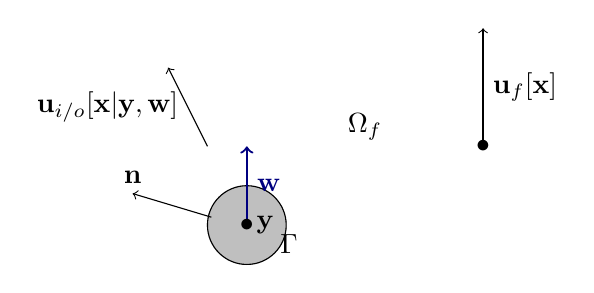
\begin{tikzpicture}
        \filldraw[ gray!50!white](0,0)circle (0.5);
        \draw(0,0)circle (0.5)node[right,below]{   $\;\;\;\;\;\;\;\;\;\;\;\Gamma$};
        \draw[->,blue!50!black,thick](0,0)--++(0,1)node[midway,right]{$\textbf{w}$};
        \draw (0,0)node{$\bullet$}node[right]{$\textbf{y}$};
        \draw[->] (-0.45,0.1)--++(-1,0.3)node[above]{$\textbf{n}$};
        \draw[->](-0.5,1)--++(-0.5,1)node[midway,left]{$\textbf{u}_{i/o}[\textbf{x}|\textbf{y},\textbf{w}]$};
        \draw[->] (3,1)node{$\bullet$}--++(0,1.5)node[right,midway]{$\textbf{u}_f[\textbf{x}]$};
        \draw (1.5,1.25)node{$\Omega_f$};
    \end{tikzpicture} 
    \caption{Representation of the problem parameters. $\textbf{u}_{o/i}[\textbf{x},\textbf{y}]+\textbf{u}_f$ is the complete velocity field generated by a test particle positioned at \textbf{y} while \textbf{u} corresponds to the disturbance velocity field.
    \textbf{n} is the unit normal  pointing outward the droplet. }
    \label{fig:disturbance}
\end{figure}

\subsection{Finite Reynolds number equaitons}

Outside and inside the volume of the test droplet we can write the governing equations of the disturbances fields as,  
\begin{align}
    \div\bm\sigma_{o}
    &= 
    Re [
    \pddt \textbf{u}_{o}
    + \textbf{u}_{o}\cdot \grad \textbf{u}_{o}
    + \textbf{u}_{o}\cdot \grad \textbf{u}_r
    + \textbf{u}_r \cdot \grad \textbf{u}_{o}]
    = Re \textbf{f}_{o}
    \label{eq:momentum_out}
    \\
    \div \textbf{u}_{o} &= 0
\end{align}
and, 
\begin{align}
    \div\bm\sigma_{i}
    &= 
    \frac{\zeta}{\lambda}Re [
    \pddt \textbf{u}_{i}
    + \textbf{u}_{i}\cdot \grad \textbf{u}_{i}
    + \textbf{u}_{i}\cdot \grad \textbf{u}_r 
    + \textbf{u}_r \cdot \grad \textbf{u}_{i}]
    = \frac{\zeta}{\lambda}Re \textbf{f}_{i}
    \label{eq:momentum_in}
    \\
    \div \textbf{u}_{i} &= 0,
\end{align}
where we introduced the relative velocity $\textbf{u}_r = \textbf{u}_f - \textbf{w}$, with \textbf{w} the center of mass velocity of the test droplet.  
$\bm\sigma_{i/o} = -p_{i/o}\bm\delta + 2\textbf{e}_{i/o}$ with $\textbf{e}_{i/o} = \frac{1}{2}[\grad \textbf{u}_{i/o} + ^{\dagger}\grad \textbf{u}_{i/o}]$ is the dimensionless newtonian stress. 
We introduce the Reynolds number $Re = \frac{\rho_f a |\textbf{u}_r|}{\mu_f}$ based on the droplet radius $a$, the density ratio $\zeta = \rho_d / \rho_f$ and the viscosity ratio $\lambda = \mu_d / \mu_f$. 
Note that the distances have been made dimensionless using the droplet radius $a$ and the velocities by $|\textbf{u}_r|$ in the above equation. 

At the surface of the droplet ($r = 1$) the continuity of velocity and the non-deformability of the test droplet imposes, 
\begin{align}
    \textbf{u}_{i} = \textbf{u}_{o}
    && 
    \textbf{u}_{i} \cdot \textbf{n}
    =
    - \textbf{u}_r \cdot \textbf{n}
    \label{eq:normal_vel}
\end{align}
where it must be noted that both $\textbf{u}_{i}$ and $\textbf{u}$ are evaluated at the points on the surface of the droplet, hence $\textbf{u}_r$ may not always be a constant vector. 
The undisturbed or ensemble averaged shear rate of the continuous phase reads  $\textbf{e}_f =\frac{1}{2} [\grad \textbf{u}_f + ^\dagger \grad \textbf{u}_f]$. 
At the interface of the test droplet the tangential shear rate is assumed continuous, however because it is the total shear rate field (and not just $\textbf{e}_{i/o}$) that satisfy this condition, we obtain (at $r=1$),
\begin{equation}
    \mathbf{n}\cdot [\textbf{e}_{o} - \lambda \textbf{e}_{i} + (1-\lambda)\textbf{e}_f
    % - \textbf{b}
    ]\cdot (\bm\delta - \textbf{nn})
    =
    \textbf{b}\cdot (\bm\delta - \textbf{nn})
    % 0
    \label{eq:boundary_cdt_stress}
\end{equation}
with, 
\begin{equation}
    \textbf{b}
    =
    \frac{a \grad \gamma}{2 \mu_f |\textbf{u}_r|}
    \approx (a\grad) Ca^{-1}. 
\end{equation}
Note that for instance the ensemble averaged quantities $\textbf{u}_f$ and $\textbf{e}_f$ are kept general, are their values may depend on the position along the surface of the test droplet. 


% where we have introduced the relative velocity field $\textbf{U}[\textbf{x},t] = \textbf{w} - \textbf{U}_f[\textbf{x},t]$. 
Far from the test droplet it is assumed that the disturbance fields are vanishingly small hence the final requirement on $p_{o}$ and $\textbf{u}_{o}$ are, 
\begin{align*}
    \lim_{|\textbf{x}-\textbf{y}|\to\infty }\textbf{u}_{o}(\textbf{x}|\textbf{y}) = 0,
    && \lim_{|\textbf{x}-\textbf{y}|\to\infty }p_{o}(\textbf{x}|\textbf{y})= 0. 
\end{align*}
This set of equation is exactly equivalent to the one derived by \cite{maxey1983equation} \& \citet{gatignol1983faxen}. 






\subsection{Stokes flow solution for a droplet embedded in a quadratic flow}
The Reciprocal theorem requires the use of a known solution.
We call that solution the \textit{test} solution, since its only purpose is to compute the \textit{real} solution of the equations introduced above. 
We note the test velocity and stress fields $\hat{\textbf{u}}_{i/o}$ and $\hat{\bm\sigma}_{i/o}$, respectively. 

In this problem we neglect all inertial effects and consider an arbitrary quadratic flow. 
In this situation $\hat{p}_{out/in}$ and $\hat{\textbf{u}}_{out/in}$ satisfy,
\begin{align}
    \div \hat{\textbf{u}}_{i} = 0 
    && \div\hat{\bm\sigma}_{i}  = 0 
    \label{eq:momentum_in_s}
    \\
    \div \hat{\textbf{u}}_{o} = 0 
    &&\div\hat{\bm\sigma}_{o}  = 0 
    \label{eq:momentum_out_s}
\end{align}
with the boundary conditions, 
\begin{equation}
    \lim_{|\textbf{x}-\textbf{y}|\to \infty}(\hat{\textbf{u}}_{o},p_{o}) = 0 
\end{equation}
and (at $r=1$),
\begin{align}
    \hat{\textbf{u}}_{i} &= \hat{\textbf{u}}_{o}\\
    \hat{\textbf{u}}_{i} \cdot \textbf{n} &= - \hat{\textbf{u}}_r \cdot \textbf{n}
    \label{eq:normal_vel_s}
    \\
    \mathbf{n}\cdot [\hat{\textbf{e}}_{o} - \lambda \hat{\textbf{e}}_{i} + (1-\lambda) \hat{\textbf{e}}_f
    % - \hat{\textbf{b}}
    ]\cdot (\bm\delta - \textbf{nn})
    &=
    \hat{\textbf{b}}\cdot (\bm\delta - \textbf{nn})
    % 0
\end{align}
where we introduced $\hat{\textbf{u}}_r = \hat{\textbf{u}}_f - \textbf{w}$ as the ensemble or undisturbed velocity field of the test problem, similarly $\hat{\textbf{e}}_f$ is the undisturbed stress of the test problem. 
In the problem considered here it is assumed that $\hat{\textbf{u}}_f$ varies very slowly compared to the droplet radius, on which we evaluate these fields. 
Additionally, because we considered a general quadratic background flow we introduce the relation, 
\begin{align}
    \hat{\textbf{u}}_r(\textbf{y}+ \textbf{r}) 
    &=  \hat{\textbf{u}}_r|_{\textbf{x}=\textbf{y}}
    +  \textbf{r} \cdot  \grad\hat{\textbf{u}}_f|_{\textbf{x}=\textbf{y}}
    +  \frac{1}{2}\textbf{rr} \cdot  \grad\grad\hat{\textbf{u}}_f|_{\textbf{x}=\textbf{y}}
    % + \ldots
    \label{eq:ufinfinity}
    \\
    \hat{\textbf{e}}_f(\textbf{y}+\textbf{r})
    &=   
    \hat{\textbf{e}}_f|_{\textbf{x}=\textbf{y}}
    + \textbf{r} \cdot  \grad \hat{\textbf{e}}_f|_{\textbf{x}=\textbf{y}}
    % + \frac{1}{2}\textbf{rr} \cdot  \grad\grad \bm\tau_f|_{\textbf{x}=0}
    % + \ldots
\end{align}
where $\textbf{y}+ \textbf{r}$ represents a point on the surface of the test droplet. 
Note that \textbf{w} is not function of \textbf{x}, hence $\grad \hat{\textbf{u}}_r = \grad \hat{\textbf{u}}_f$  in \ref{eq:ufinfinity}. 


Using the standard procedure of spherical harmonics we can stipulate that, \citep{leal2007advanced,raja2010inertial,nadim1991motion},
% \begin{align*}
%     \begin{pmatrix}
%         \hat{\textbf{u}}_{o}\\
%         \hat{p}_{o}\\
%         \hat{\textbf{u}}_{i}\\
%         \hat{p}_{i}
%     \end{pmatrix}
%     =
%     \begin{pmatrix}
%         \mathcal{U}_{o}^{(1)} + \mathcal{U}_{o}^{(2)}\cdot \grad + \frac{1}{2}\mathcal{U}_{o}^{(3)} :\grad\grad \\
%         \mathcal{P}_{o}^{(1)} + \mathcal{P}_{o}^{(2)}\cdot \grad + \frac{1}{2}\mathcal{P}_{o}^{(3)} :\grad\grad \\
%         \mathcal{U}_{i}^{(1)} + \mathcal{U}_{i}^{(2)}\cdot \grad + \frac{1}{2}\mathcal{U}_{i}^{(3)} :\grad\grad \\
%         \mathcal{P}_{i}^{(1)} + \mathcal{P}_{i}^{(2)}\cdot \grad + \frac{1}{2}\mathcal{P}_{i}^{(3)} :\grad\grad \\
%     \end{pmatrix}
%     \cdot 
%     \hat{\textbf{u}}_r|_{\textbf{x}=\textbf{y}}
% \end{align*}
\begin{align*}
    \begin{pmatrix}
        \hat{\textbf{u}}_{o}\\
        \hat{p}_{o}\\
        \hat{\textbf{u}}_{i}\\
        \hat{p}_{i}
    \end{pmatrix}
    =
    \begin{pmatrix}
        \mathcal{U}_{o}^{(1)} + \mathcal{U}_{o}^{(2)}\cdot \grad + \mathcal{U}_{o}^{(3)} :\grad\grad &
        \mathcal{U}_{o}^\text{(b-1)} + \mathcal{U}_{o}^\text{(b-2)}\cdot \grad + \mathcal{U}_{o}^\text{(b-3)} :\grad\grad \\
        \mathcal{P}_{o}^{(1)} + \mathcal{P}_{o}^{(2)}\cdot \grad + \mathcal{P}_{o}^{(3)} :\grad\grad &
        \mathcal{P}_{o}^\text{(b-1)} + \mathcal{P}_{o}^\text{(b-2)}\cdot \grad + \mathcal{P}_{o}^\text{(b-3)} :\grad\grad \\
        \mathcal{U}_{i}^{(1)} + \mathcal{U}_{i}^{(2)}\cdot \grad + \mathcal{U}_{i}^{(3)} :\grad\grad &
        \mathcal{U}_{i}^\text{(b-1)} + \mathcal{U}_{i}^\text{(b-2)}\cdot \grad + \mathcal{U}_{i}^\text{(b-3)} :\grad\grad \\
        \mathcal{P}_{i}^{(1)} + \mathcal{P}_{i}^{(2)}\cdot \grad + \mathcal{P}_{i}^{(3)} :\grad\grad &
        \mathcal{P}_{i}^\text{(b-1)} + \mathcal{P}_{i}^\text{(b-2)}\cdot \grad + \mathcal{P}_{i}^\text{(b-3)} :\grad\grad \\
    \end{pmatrix}
    \cdot 
    \begin{pmatrix}
        \hat{\textbf{u}}_r\\
        \hat{\textbf{b}}
    \end{pmatrix}
\end{align*}
The tensor $\mathcal{U}_{o}^{(1)},\mathcal{U}_{i}^{(1)},\mathcal{P}_{o}^{(1)}$  and $\mathcal{P}_{i}^{(1)}$ represent the effect of uniform relative translation $\hat{\textbf{u}}_r$ on the disturbance fields.
Hence these expressions correspond to the Hadamard-Ribczynski solution \citep{pozrikidis1992boundary,kim2013microhydrodynamics}. 
The dependency with the mean gradient velocity $\grad \hat{\textbf{u}}_f|_{\textbf{x}=\textbf{y}}$, evaluated at the center of mass of the test droplet, is defined through the tensor $\mathcal{U}_{o}^{(2)},\mathcal{U}_{i}^{(2)},\mathcal{P}_{o}^{(2)}$ and $\mathcal{P}_{i}^{(2)}$.
The solution for these tensors is derived in \citet{rallison1978note,leal2007advanced,raja2010inertial}. 
Finally the disturbance field of a droplet in the quadratic flow, $\grad\grad \hat{\textbf{u}}_f|_{\textbf{x}=\textbf{y}}$, is defined with the tensors $\mathcal{U}_{o}^{(3)},\mathcal{U}_{i}^{(3)},\mathcal{P}_{o}^{(3)}$ and $\mathcal{P}_{i}^{(3)}$.
The definition of the former tensors can be found in \citet{nadim1991motion}.


\subsection{Point source solution}



Following \citet{stone2001inertial} we also consider the test problem of a point source of strength $Q$ located at the center of the sphere (\textbf{y}).
In this case the test velocity  and stress fields, reads\citep{pozrikidis2011introduction,pozrikidis1992boundary}, 
\begin{align}
    \hat{\textbf{u}}_{o/i} = \frac{Q}{4\pi} \frac{\textbf{r}}{r^3}
    && \hat{\bm\sigma}_{o/i} = \mu_f \frac{Q}{2\pi}\left(
        \frac{\bm\delta}{r^3}
        - \frac{3 \textbf{rr}}{r^5}
    \right)
    \label{eq:point_source}
\end{align}
Note that this expression is valid throughout the domain excluding the point $\textbf{r} =  \textbf{x} -  \textbf{y} = 0$, hence we may use either the subscript $o$ or $i$. 
In the previous test problem $\div \hat{\textbf{u}}_f= 0$ (in opposition to \ref{eq:point_source}), thus the previous solution is unable to provide a formula for the trace of the first moment using the reciprocal theorem \citep{stone2001inertial}.

\tb{Metrre vec normal }


\section{Reciprocal theorem for droplets}

We now demonstrate how to derive the reciprocal theorem for droplets.
Note that a similar derivation to what is presented here may be found in \citet{lovalenti1993force,raja2010inertial}, however we hope to provide some clarification by exposing a detailed and simpler demonstration.  

The derivation of the general formula goes into three steps. 

\subsection{First step:}
We first take the dot product of \ref{eq:momentum_out} with $\hat{\textbf{u}}_{o}$, and the dot product of \ref{eq:momentum_out_s} with $\textbf{u}_{o}$, subtracting both expression gives, 
\begin{equation}
    \div (\bm\sigma_{o}\cdot \hat{\textbf{u}}_o)
    % - \bm\sigma_o :\grad \hat{\textbf{u}}_o
    % \hat{\textbf{u}}_{o} \cdot (\div \bm\sigma_{o})
    =
    \div (\hat{\bm\sigma}_{o}\cdot \textbf{u}_o)
    % - \hat{\bm\sigma}_o :\grad \textbf{u}_o
    + Re (\hat{\textbf{u}}_{o}\cdot \textbf{f}_{o}). 
    \label{eq:first_step_out}
\end{equation}
To derive this relation we used the fact that $\bm\sigma_o :\grad \hat{\textbf{u}}_o = 2\textbf{e}_o :\grad \hat{\textbf{u}}_o = 2{\textbf e}_o : \hat{\textbf e}_o$, and  $\hat{\bm\sigma}_o :\grad {\textbf{u}}_o = 2\hat{\textbf{e}}_o : \textbf{e}$, leading to $\bm\sigma_o :\grad \hat{\textbf{u}}_o = \hat{\bm\sigma}_o :\grad {\textbf{u}}_o$. 
This simplification is the reason why the complete knowledge of the velocity field becomes unnecessary with the reciprocal theorem when $\textbf{f}_o = 0$.
Consequently, the  efficiency of the reciprocal theorem is rooted in the commutativity of the operation $\textbf e:\hat{\textbf e}$. 
Integrating this expression on the whole domain $\Omega_{o}$, and injecting the relations $\textbf{u}_o = \textbf{u}_o+\textbf{u}_r-\textbf{u}_r$ and $\hat{\textbf{u}}_o = \hat{\textbf{u}}_o+\hat{\textbf{u}}_r-\hat{\textbf{u}}_r$ gives, 
\begin{equation}
    \intS[p]{\hat{\textbf{u}}_{r} \cdot  \bm\sigma_{o}\cdot \textbf{n}}
    - 2\intS[p]{(\hat{\textbf{u}}_{o} + \hat{\textbf{u}}_r) \cdot  \textbf e_{o}\cdot \textbf{n}}
    =
    \intS[p]{\textbf{u}_{r}\cdot \hat{\bm\sigma}_{o}\cdot \textbf{n}}
    - 2\intS[p]{(\textbf{u}_{o} + \textbf{u}_r)\cdot \hat{\textbf e}_{o}\cdot \textbf{n}}
    + 
    Re\intO[o]{\hat{\textbf{u}}_{o}\cdot \textbf{f}_{o}}.
    \label{eq:int_first_step}
\end{equation}
Where we used the relation, $(\hat{\textbf{u}}_{o} + \hat{\textbf{u}}_r) \cdot  \bm\sigma_{o}\cdot \textbf{n} = 2 (\hat{\textbf{u}}_{o} + \hat{\textbf{u}}_r) \cdot  \textbf e_{o}\cdot \textbf{n}$, allowed because of \ref{eq:normal_vel_s}, and because $(\hat{\textbf{u}}_{o} + \hat{\textbf{u}}_r) = (\bm\delta - \textbf{nn})\cdot (\hat{\textbf{u}}_{o} + \hat{\textbf{u}}_r)$ on the surface of the test droplet. 
Similar considerations lead to $({\textbf{u}}_{o} + {\textbf{u}_r}) \cdot  \hat{\bm\sigma}_{o}\cdot \textbf{n} =2  ({\textbf{u}}_{o} + {\textbf{u}_r}) \cdot  \hat{\textbf e}_{o}\cdot \textbf{n}$. 
\ref{eq:int_first_step} is the correct expression of the reciprocal theorem to use if one consider solid particles.
Indeed, in that case $\hat{\textbf{u}}_{o}$ is imposed by the no-slip boundary condition at the particle interface, hence leading directly to a formula for the force traction at the surface of the solid particle. 
For fluid particles few more steps are required. 

\subsection{Second step:}

We now take the dot product of \ref{eq:momentum_in} with $(\hat{\textbf{u}}_i + \hat{\textbf{u}}_r)$ and of \ref{eq:momentum_in_s} with $(\textbf{u}_i+ \textbf{u}_r)$, subtracting both expression leads to, 
\begin{equation}
    \div [\bm\sigma_{i}\cdot (\hat{\textbf{u}}_i+\hat{\textbf{u}}_r)]
    - 2\textbf{e}_i : \hat{\textbf{e}}_f
    % \hat{\textbf{u}}_{i} \cdot (\div \bm\sigma_{i})
    =
    \div [\hat{\bm\sigma}_{i}\cdot (\textbf{u}_i+\textbf{u}_r)]
    - 2\hat{\textbf{e}}_i :\textbf{e}_f
    + \frac{\zeta}{\lambda} Re (\hat{\textbf{u}}_i+\hat{\textbf{u}}_r)\cdot \textbf{f}_{i}. 
    \label{eq:second_step_out}
\end{equation}
where we used the relation, $- \bm\sigma_i :\grad (\hat{\textbf{u}}_i+\hat{\textbf{u}}_r)+ \hat{\bm\sigma}_i :\grad ({\textbf{u}}_i+{\textbf{u}}_r) =
- 2\textbf{e}_i :\hat{\textbf{e}}_f + 2\hat{\textbf{e}}_i :\textbf{e}_f$. 
% We recall that $\hat{\bm\tau}_f$ and $\bm\tau_f$ correspond to the ensemble averaged stress fields of the test problem and true problem, respectively. 
Integrating this relation over the domain $\Omega_i$, and using the divergence theorem, as well as similar simplifications used in \ref{eq:int_first_step}, gives, 
\begin{equation}
    \intS[p]{ (\hat{\textbf{u}}_i+\hat{\textbf{u}}_r)\cdot \textbf{e}_{i}\cdot\textbf{n}}
    - \intO[i]{\textbf{e}_i : \hat{\textbf{e}}_f}
    =
    \intS[p]{ (\textbf{u}_i+\textbf{u}_r)\cdot\hat{\textbf{e}}_{i}\cdot \textbf{n}}
    - \intO[i]{\hat{\textbf{e}}_i :\textbf{e}_f}
    + \frac{\zeta}{2\lambda} Re \intO{(\hat{\textbf{u}}_i+\hat{\textbf{u}}_r)\cdot \textbf{f}_{i}} 
    \label{eq:second_step_int}
\end{equation}
Because $(\hat{\textbf{u}}_i+\hat{\textbf{u}}_r)\cdot (\bm\delta-\textbf{nn}) = (\hat{\textbf{u}}_i+\hat{\textbf{u}}_r)$, multiplying \ref{eq:boundary_cdt_stress} by $(\hat{\textbf{u}}_i+\hat{\textbf{u}}_r)$ gives the appropriate boundary condition for the first integral on the left-hand side of \ref{eq:second_step_int}, namely,
\begin{equation}
    \mathbf{n}\cdot [
        \textbf{e}_{o} - \lambda \textbf{e}_i 
        + (1 -\lambda) \textbf{e}_f
        % - \textbf{b}
        ]\cdot (\hat{\textbf{u}}_{i/o}+\hat{\textbf{u}}_r)
        =
        \textbf{b}\cdot (\hat{\textbf{u}}_{i/o}+\hat{\textbf{u}}_r)
    \label{eq:boundary_with_the_velocity}
\end{equation}
with a similar relation for the test problem boundary condition and $({\textbf{u}}_{i/o}+{\textbf{u}}_r)$ in the first integral on the right-hand side of \ref{eq:second_step_int}. 

Adding \ref{eq:int_first_step} and \ref{eq:second_step_int} times $\lambda$, while using the boundary condition given by \ref{eq:boundary_with_the_velocity} leads to the expression,
\begin{multline}
    \intS[p]{\hat{\textbf{u}}_{r} \cdot  \bm\sigma_{o}\cdot \textbf{n}}
    -\lambda \intO[i]{2\textbf{e}_i : \hat{\textbf{e}}_f}
    - (1-\lambda) \intS[p]{2(\textbf{u}_{i} + \textbf{u}_r)\cdot \hat{\textbf{e}}_f\cdot \textbf{n}}
    + \intS[p]{2(\textbf{u}_{i} + \textbf{u}_r)\cdot \hat{\textbf{b}}}
    \\
    =
    \intS[p]{\textbf{u}_{r}\cdot \hat{\bm\sigma}_{o}\cdot \textbf{n}}
    - \lambda \intO[i]{2\hat{\textbf{e}}_i :\textbf{e}_f}
    - (1-\lambda) \intS[p]{2(\hat{\textbf{u}}_{i} + \hat{\textbf{u}}_r) \cdot  \textbf{e}_f \cdot \textbf{n}}
    + \intS[p]{2(\hat{\textbf{u}}_{i} + \hat{\textbf{u}}_r) \cdot  \textbf{b}}
    \\ 
    + \zeta Re \intO{(\hat{\textbf{u}}_i+\hat{\textbf{u}}_r)\cdot \textbf{f}_{i}} 
    + Re\intO[o]{\hat{\textbf{u}}_{o}\cdot \textbf{f}_{o}}.
    \label{eq:int_third_step}
\end{multline}

\subsection{Final step:}

To obtain the `final form' of the reciprocal theorem we proceed by noting that the last two terms on the left-hand side  of \ref{eq:int_third_step} may be combined upon using the divergence theorem on the third term, and using the relation, 
\begin{equation}
    - \lambda \textbf{e}_i : \hat{\textbf{e}}_f
    - (1-\lambda)\div [\hat{\textbf{e}_f} \cdot (\textbf{u}_i + \textbf{u}_r)]
    =
    % - \lambda \textbf{e}_i : \hat{\textbf{e}_f}
    % - (1-\lambda) \hat{\textbf{e}_f}:(\textbf{e}_i + \textbf{e}_f)
    - \textbf{e}_i : \hat{\textbf{e}_f}
    - (1-\lambda) \hat{\textbf{e}_f}:\textbf{e}_f
    - (1-\lambda)\div \hat{\textbf{e}_f} \cdot (\textbf{u}_i + \textbf{u}_r).
    \label{eq:tricks_two}
\end{equation}
One can also derive the same manipulation on the second and third term on the right-hand side of \ref{eq:int_third_step}, namely,
\begin{equation}
    - \lambda \hat{\textbf{e}}_i : {\textbf{e}}_f
    - (1-\lambda)\div [{\textbf{e}_f} \cdot (\hat{\textbf{u}}_i + \hat{\textbf{u}}_r)]
    =
    % - \lambda \textbf{e}_i : \hat{\textbf{e}_f}
    % - (1-\lambda) \hat{\textbf{e}_f}:(\textbf{e}_i + \textbf{e}_f)
    - \hat{\textbf{e}_i} : {\textbf{e}_f}
    - (1-\lambda) \hat{\textbf{e}_f}:\textbf{e}_f
    - (1-\lambda)\div {\textbf{e}_f} \cdot (\hat{\textbf{u}}_i + \hat{\textbf{u}}_r)
    \label{eq:tricks_one}
\end{equation}
Because the product $\hat{\textbf{e}_i} : {\textbf{e}_f}$ is commutative, the second term of \ref{eq:tricks_one} and \ref{eq:tricks_two} cancel each other in the final expression.  
Injecting both \ref{eq:tricks_one} and \ref{eq:tricks_two} in \ref{eq:int_third_step} leads to the final form of the reciprocal theorem for droplets, 
\begin{multline}
    \intS[p]{\hat{\textbf{u}}_{r} \cdot  \bm\sigma_{o}\cdot \textbf{n}}
    - \intO[i]{2\textbf{e}_i : \grad\hat{\textbf{u}}_f}
    - (1-\lambda) \intO[p]{(\textbf{u}_{i} + \textbf{u}_r)\cdot \grad^2 \hat{\textbf{u}}_f}
    + \intS[p]{2(\textbf{u}_{i} + \textbf{u}_r)\cdot \hat{\textbf{b}}}
    \\
    =
    \intS[p]{\textbf{u}_{r}\cdot \hat{\bm\sigma}_{o}\cdot \textbf{n}}
    - \intO[i]{2\hat{\textbf{e}}_i :\grad\textbf{u}_f}
    - (1-\lambda) \intO[p]{(\hat{\textbf{u}}_{i} + \hat{\textbf{u}}_r) \cdot \grad^2 \textbf{u}_f }
    + \intS[p]{2(\hat{\textbf{u}}_{i} + \hat{\textbf{u}}_r) \cdot  \textbf{b}}
    \\ 
    + \zeta Re \intO{(\hat{\textbf{u}}_i+\hat{\textbf{u}}_r)\cdot \textbf{f}_{i}} 
    + Re\intO[o]{\hat{\textbf{u}}_{o}\cdot \textbf{f}_{o}}.
    \label{eq:int_final_step}
\end{multline}
% \begin{multline}
%     \intS[p]{\hat{\textbf{u}}_{r} \cdot  \bm\sigma_{o}\cdot \textbf{n}}
%     - \intO[i]{2\textbf{e}_i : \hat{\textbf{e}}_f}
%     + (\lambda-1) \intO[p]{2(\textbf{u}_{i} + \textbf{u}_r)\cdot \div \hat{\textbf{e}}_f}
%     \\
%     =
%     \intS[p]{\textbf{u}_{r}\cdot \hat{\bm\sigma}_{o}\cdot \textbf{n}}
%     - \intO[i]{2\hat{\textbf{e}}_i :\textbf{e}_f}
%     + (\lambda-1) \intO[p]{2(\hat{\textbf{u}}_{i} + \hat{\textbf{u}}_r) \cdot \div   \textbf{e}_f }
%     \\ 
%     + \zeta Re \intO{(\hat{\textbf{u}}_i+\hat{\textbf{u}}_r)\cdot \textbf{f}_{i}} 
%     + Re\intO[o]{\hat{\textbf{u}}_{o}\cdot \textbf{f}_{o}}.
%     \label{eq:int_final_step}
% \end{multline}
Where we used the relations, $2{\textbf{e}_i} : \hat{\textbf{e}_f}= 2{\textbf{e}_i} : {\grad\textbf{u}_f}$ and $\div\textbf{e}_f = \frac{1}{2}\grad^2 \textbf{u}_f$ because the background flow is divergence free. 
Upon making the good choice for $(\hat{\textbf{e}}_f, \hat{\textbf{u}}_r)$, one recover on the left-hand side of \ref{eq:int_final_step} the expression of the drag force and the first, second and higher moments present in \ref{eq:f_alpha} and \ref{eq:def_sigma_eff_f}, respectively. 
The note that on the right-hand side of \ref{eq:int_final_step} all the terms, are either, known quantities from our test problem ($\hat{\bm\sigma}_{o},\hat{\textbf{e}}_i, \hat{\textbf{u}}_{i/o/r}$), or far-field condition of our `real' problem ($\textbf{e}_f,\textbf{u}_r$). 
However, one exception remain, that is the inertial term $\textbf{f}_{i/o}$ to be evaluated in the whole domain $\Omega$, which is a function of the unknown velocity field $\textbf{u}_{i/o}$. 

Hence, to compute the right-hand-side \ref{eq:int_final_step} one must proceed by applying some approximation allowing us to obtain the last two terms of \ref{eq:int_final_step}. 
This is the subject of the next section. 




\section{Moments of force on a droplet}


\subsection{General formula for the force, first and second moments}
The drag force, Stresslet and second moment of forces are obtained by selecting the following quantity for the test problem, 
\begin{align}
    \hat{\textbf{u}}_r = \hat{\textbf{u}}_r|_{\textbf{x}=\textbf{y}} 
    && 
    \hat{\textbf{b}} = 0 
    && 
    \hat{\textbf{u}}_{o/i} = \mathcal{U}_{o/i}^{(1)}\cdot \hat{\textbf{u}}_r|_{\textbf{x}=\textbf{y}} 
    && 
    \hat{\bm\sigma}_{o/i} = \mathcal{S}_{o/i}^{(1)}\cdot \hat{\textbf{u}}_r|_{\textbf{x}=\textbf{y}} \\
    \hat{\textbf{u}}_r =\textbf{r}\cdot  \grad \textbf{u}_f|_{\textbf{x}=\textbf{y}} 
    && 
    \hat{\textbf{b}} = 0 
    && 
    \hat{\textbf{u}}_{o/i} = \mathcal{U}_{o/i}^{(2)} : \grad\hat{\textbf{u}}_f|_{\textbf{x}=\textbf{y}} 
    && 
    \hat{\bm\sigma}_{o/i} = \mathcal{S}_{o/i}^{(2)} : \grad\hat{\textbf{u}}_f|_{\textbf{x}=\textbf{y}} \\
    \hat{\textbf{u}}_r =\frac{1}{2}\textbf{rr}\cdot  \grad\grad \textbf{u}_f|_{\textbf{x}=\textbf{y}} 
    && 
    \hat{\textbf{b}} = 0 
    && 
    \hat{\textbf{u}}_{o/i} = \mathcal{U}_{o/i}^{(3)} \vdots \grad\grad\hat{\textbf{u}}_f|_{\textbf{x}=\textbf{y}} 
    && 
    \hat{\bm\sigma}_{o/i} = \mathcal{S}_{o/i}^{(3)} \vdots \grad\grad\hat{\textbf{u}}_f|_{\textbf{x}=\textbf{y}} 
    \label{eq:test_prob1}
\end{align}
which correspond to the velocity and stress fields condition of an isolated translating drop.
Because $\hat{\textbf{u}}_r|_{\textbf{x}=\textbf{y}} $ is arbitrary, injecting \ref{eq:test_prob1} into \ref{eq:int_final_step} gives the formula
\begin{multline}
    \intS[p]{\bm\sigma_{o}\cdot \textbf{n}}
    =
    \intS[p]{\textbf{u}_{r}\cdot \mathcal{S}_o^{(1)} \cdot \textbf{n}}
    - \intO[i]{ \mathcal{S}_{i}^{(1)} :\grad\textbf{u}_f}
    - (1-\lambda) \intO[p]{(\mathcal{U}_{i}^{(1)} + \bm\delta) \cdot \grad^2   \textbf{u}_f }
    \\ 
    + \intS[p]{2(\mathcal{U}_{i}^{(1)} + \bm\delta) \cdot  \textbf{b}}
    + \zeta Re \intO{(\mathcal{U}_{i}^{(1)} + \bm\delta)\cdot \textbf{f}_{i}} 
    + Re\intO[o]{\mathcal{U}_{o}^{(1)}\cdot \textbf{f}_{o}},
\end{multline}
\begin{multline}
    \intS[p]{\textbf{r}  \bm\sigma_{o}\cdot \textbf{n}}
    - \intO[i]{2\textbf{e}_i}
    =
    \intS[p]{\textbf{u}_{r}\cdot  \mathcal{S}_o^{(2)}\cdot \textbf{n}}
    - \intO[i]{ \mathcal{S}_i^{(2)} :\grad\textbf{u}_f}
    - (1-\lambda) \intO[p]{(\mathcal{U}_{i}^{(2)}  + \textbf{r}\bm\delta) \cdot \grad^2   \textbf{u}_f }
    \\ 
    + \intS[p]{2(\mathcal{U}_{i}^{(2)} + \textbf{r}\bm\delta) \cdot  \textbf{b}}
    + \zeta Re \intO{(\mathcal{U}_{i}^{(2)}  + \textbf{r}\bm\delta)\cdot \textbf{f}_{i}} 
    + Re\intO[o]{\mathcal{U}_{o}^{(2)}\cdot \textbf{f}_{o}},
\end{multline}
\begin{multline}
    \intS[p]{\textbf{rr}  \bm\sigma_{o}\cdot \textbf{n}}
    - \intO[i]{2\textbf{re}_i }
    % - (1-\lambda) \intO[p]{2(\textbf{u}_{i} + \textbf{u}_r):\bm\delta}
    % \\
    =
    \intS[p]{\textbf{u}_{r}\cdot \mathcal{S}_o^{(3)}\cdot \textbf{n}}
    - \intO[i]{\mathcal{S}_i^{(3)} :\grad\textbf{u}_f}
    - (1-\lambda) \intO[p]{(\mathcal{U}_{i}^{(3)} + \textbf{rr}\bm\delta) \cdot \grad^2 \textbf{u}_f }\\
    + \intS[p]{2(\mathcal{U}_{i}^{(3)} + \textbf{rr}\bm\delta) \cdot  \textbf{b}}
    + \zeta Re \intO{(\mathcal{U}_{i}^{(3)} + \textbf{rr}\bm\delta)\cdot \textbf{f}_{i}} 
    + Re\intO[o]{\mathcal{U}_{o}^{(3)} \cdot \textbf{f}_{o}}.
\end{multline}
Note that the integral of $\textbf{u}_o + \textbf{u}_r = \textbf{u}_o+\textbf{u}_f - \textbf{w}$, hence it correspond to the integral of the velocity relative to the center of mass velocity over the droplet volume. Therefore this term vanish. 

Now it is left to specify in which circumstances we want to compute the drag force and other moments, then fixing the boundaries conditions defined by $\textbf{u}_r$ and the higher gradients. 
Note that we could present the closures all at once for an arbitrary flow however it turns out to be clearer that way. 

\subsection{General formulation for the internal shear integrals}

\begin{align}
    \hat{\textbf{u}}_r = 0
    && 
    \hat{\textbf{b}} = \textbf{b}|_{\textbf{x}=\textbf{y}} 
    && 
    \hat{\textbf{u}}_{o/i} = \mathcal{U}_{o/i}^\text{(1-b)}\cdot  \textbf{b}|_{\textbf{x}=\textbf{y}} 
    && 
    \hat{\bm\sigma}_{o/i} = \mathcal{S}_{o/i}^{(1-b)}\cdot \textbf{b}|_{\textbf{x}=\textbf{y}} \\
    \hat{\textbf{u}}_r = 0
    && 
    \hat{\textbf{b}} = \textbf{r}\cdot \grad\textbf{b}|_{\textbf{x}=\textbf{y}} 
    && 
    \hat{\textbf{u}}_{o/i} = \mathcal{U}_{o/i}^\text{(2-b)}:  \grad\textbf{b}|_{\textbf{x}=\textbf{y}} 
    && 
    \hat{\bm\sigma}_{o/i} = \mathcal{S}_{o/i}^{(2-b)}:\grad \textbf{b}|_{\textbf{x}=\textbf{y}} \\
    \hat{\textbf{u}}_r = 0
    && 
    \hat{\textbf{b}} = \frac{1}{2}\textbf{rr} : \grad\grad\textbf{b}|_{\textbf{x}=\textbf{y}} 
    && 
    \hat{\textbf{u}}_{o/i} = \mathcal{U}_{o/i}^\text{(3-b)}\vdots  \grad\grad\textbf{b}|_{\textbf{x}=\textbf{y}} 
    && 
    \hat{\bm\sigma}_{o/i} = \mathcal{S}_{o/i}^{(3-b)}\vdots\grad\grad \textbf{b}|_{\textbf{x}=\textbf{y}} \\
    \label{eq:test_prob1}
\end{align}

which gives, 
\begin{multline}
    \intS[p]{2(\textbf{u}_{i} + \textbf{u}_r)}
    =
    \intS[p]{\textbf{u}_{r}\cdot \mathcal{S}^\text{(1-b)}_{o/i} \cdot \textbf{n}}
    - \intO[i]{\mathcal{S}^\text{(1-b)}_{o/i} :\grad\textbf{u}_f}
    - (1-\lambda) \intO[p]{\mathcal{U}^\text{(1-b)}_{i} \cdot \grad^2 \textbf{u}_f }\\
    + \intS[p]{2 \mathcal{U}^\text{(1-b)}_{i}  \cdot  \textbf{b}}
    + \zeta Re \intO{\mathcal{U}^\text{(1-b)}_{i} \cdot \textbf{f}_{i}} 
    + Re\intO[o]{\mathcal{U}^\text{(1-b)}_{o}\cdot \textbf{f}_{o}}.
    \label{eq:int_final_step}
\end{multline}
\begin{multline}
    \intS[p]{2(\textbf{u}_{i} + \textbf{u}_r)\textbf{r}}
    =
    \intS[p]{\textbf{u}_{r}\cdot \mathcal{S}^\text{(2-b)}_{o/i} \cdot \textbf{n}}
    - \intO[i]{\mathcal{S}^\text{(2-b)}_{o/i} :\grad\textbf{u}_f}
    - (1-\lambda) \intO[p]{\mathcal{U}^\text{(2-b)}_{i} \cdot \grad^2 \textbf{u}_f }\\
    + \intS[p]{2\mathcal{U}^\text{(2-b)}_{i} \cdot  \textbf{b}}
    % \\ 
    + \zeta Re \intO{\mathcal{U}^\text{(2-b)}_{i} \cdot \textbf{f}_{i}} 
    + Re\intO[o]{\mathcal{U}^\text{(2-b)}_{o}\cdot \textbf{f}_{o}}.
    \label{eq:un}
\end{multline}
% \begin{multline}
%     \intS[p]{\hat{\textbf{u}}_{r} \cdot  \bm\sigma_{o}\cdot \textbf{n}}
%     - \intO[i]{2\textbf{e}_i : \grad\hat{\textbf{u}}_f}
%     - (1-\lambda) \intO[p]{(\textbf{u}_{i} + \textbf{u}_r)\cdot \grad^2 \hat{\textbf{u}}_f}
%     + \intS[p]{2(\textbf{u}_{i} + \textbf{u}_r)\cdot \hat{\textbf{b}}}
%     \\
%     =
%     \intS[p]{\textbf{u}_{r}\cdot \hat{\bm\sigma}_{o}\cdot \textbf{n}}
%     - \intO[i]{2\hat{\textbf{e}}_i :\grad\textbf{u}_f}
%     - (1-\lambda) \intO[p]{(\hat{\textbf{u}}_{i} + \hat{\textbf{u}}_r) \cdot \grad^2 \textbf{u}_f }
%     + \intS[p]{2(\hat{\textbf{u}}_{i} + \hat{\textbf{u}}_r) \cdot  \textbf{b}}
%     \\ 
%     + \zeta Re \intO{(\hat{\textbf{u}}_i+\hat{\textbf{u}}_r)\cdot \textbf{f}_{i}} 
%     + Re\intO[o]{\hat{\textbf{u}}_{o}\cdot \textbf{f}_{o}}.
% \end{multline}
where the forcing term of this problem is determined by the imposed flow

\subsection{Uniform translation without Marangoni forces}
In the `true' problem we consider in the first place a uniform translation situation.
Such that, 
\begin{align*}
    \textbf{u}_r = \textbf{u}_r|_{\textbf{x}=\textbf{y}} . 
\end{align*}
In this particlar cases we obtain the following formulas,
\begin{multline}
    \intS[p]{\bm\sigma_{o}\cdot \textbf{n}}
    =
    \textbf{u}_{r}\cdot\intS[p]{ \mathcal{S}_o^{(1)} \cdot \textbf{n}}
    % - \intO[i]{ \mathcal{S}_{i}^{(1)} :\grad\textbf{u}_f}
    % + (\lambda-1) \intO[p]{(\mathcal{U}_{i}^{(1)} + \bm\delta) \cdot \grad^2   \textbf{u}_f }\\ 
    + \zeta Re \intO{(\mathcal{U}_{i}^{(1)} + \bm\delta)\cdot \textbf{f}_{i}} 
    + Re\intO[o]{\mathcal{U}_{o}^{(1)}\cdot \textbf{f}_{o}},\\
    \intS[p]{\textbf{r}  \bm\sigma_{o}\cdot \textbf{n}}
    - \intO[i]{2\textbf{e}_i}
    =
    \textbf{u}_{r}\cdot\intS[p]{  \mathcal{S}_o^{(2)}\cdot \textbf{n}}
    % - \intO[i]{ \mathcal{S}_i^{(2)} :\grad\textbf{u}_f}
    % + (\lambda-1) \intO[p]{(\mathcal{U}_{i}^{(2)}  + \textbf{r}\bm\delta) \cdot \grad^2   \textbf{u}_f }
    + \zeta Re \intO{(\mathcal{U}_{i}^{(2)}  + \textbf{r}\bm\delta)\cdot \textbf{f}_{i}} 
    + Re\intO[o]{\mathcal{U}_{o}^{(2)}\cdot \textbf{f}_{o}},\\
    \intS[p]{\textbf{rr}  \bm\sigma_{o}\cdot \textbf{n}}
    - \intO[i]{2\textbf{re}_i}
    % + (\lambda-1) \intO[p]{2(\textbf{u}_{i} + \textbf{u}_r):\bm\delta}
    % \\
    =
    \textbf{u}_{r}\cdot\intS[p]{ \mathcal{S}_o^{(3)}\cdot \textbf{n}}
    % - \intO[i]{\mathcal{S}_i^{(3)} :\grad\textbf{u}_f}\\
    % + (\lambda-1) \intO[p]{(\mathcal{U}_{i}^{(3)} + \textbf{rr}\bm\delta) \cdot \grad^2 \textbf{u}_f }
    + \zeta Re \intO{(\mathcal{U}_{i}^{(3)} + \textbf{rr}\bm\delta)\cdot \textbf{f}_{i}} 
    + Re\intO[o]{\mathcal{U}_{o}^{(3)} \cdot \textbf{f}_{o}},
\end{multline}
Additionally, one may need to compute the internal shear independently in which case he uses \ref{eq:un} 
\begin{equation}
    \intS[p]{2\textbf{u}_{i} \textbf{r}}
    =
    \textbf{u}_{r}\cdot \intS[p]{ \mathcal{S}^\text{(2-b)}_{o/i} \cdot \textbf{n}}
    % \\ 
    + \zeta Re \intO{\mathcal{U}^\text{(2-b)}_{i} \cdot \textbf{f}_{i}} 
    + Re\intO[o]{\mathcal{U}^\text{(2-b)}_{o}\cdot \textbf{f}_{o}}.
\end{equation}
Because, $\textbf{u}_r$ is constant, its contribution on
where the inertial terms become, 
\begin{equation}
    \textbf{f}_{o/i} = \pddt \textbf{u}_{o/i} + (\textbf{u}_{o/i} + \textbf{u}_r) \cdot \grad \textbf{u}_{o/i}
\end{equation}
The first term of each equation corresponds by definition to the stokes contribution drag force contribution to the droplets, the two remaining ones correspond to the inertial contributions. 

Basically the additional contribution of the first moment will be there, $\textbf{u}_r\textbf{u}_r$ regarding the other contribution it will be about that $\pddt \textbf{u}_r$ on the second moment 


\tb{ALLL THESE TERMS MUST BE COMPUTED NOW}
\subsection{Pure linear flow translation}
Now we consider that, 
\begin{equation}
    \textbf{u}_r = \textbf{r}\cdot \grad \textbf{u}_f |_{\textbf{x}=\textbf{y}}
\end{equation}

\begin{multline}
    \intS[p]{\bm\sigma_{o}\cdot \textbf{n}}
    =
    \grad \textbf{u}_f\cdot \intS[p]{\textbf{r} \mathcal{S}_o^{(1)} \cdot \textbf{n}}
    - \grad\textbf{u}_f:\intO[i]{ \mathcal{S}_{i}^{(1)}}
    \\ 
    + \zeta Re \intO{(\mathcal{U}_{i}^{(1)} + \bm\delta)\cdot \textbf{f}_{i}} 
    + Re\intO[o]{\mathcal{U}_{o}^{(1)}\cdot \textbf{f}_{o}},
\end{multline}
\begin{multline}
    \intS[p]{\textbf{r}  \bm\sigma_{o}\cdot \textbf{n}}
    - \intO[i]{2\textbf{e}_i}
    =
    \grad \textbf{u}_f\cdot \intS[p]{\textbf{r}  \mathcal{S}_o^{(2)}\cdot \textbf{n}}
    - \grad\textbf{u}_f:\intO[i]{ \mathcal{S}_i^{(2)}}
    \\ 
    + \zeta Re \intO{(\mathcal{U}_{i}^{(2)}  + \textbf{r}\bm\delta)\cdot \textbf{f}_{i}} 
    + Re\intO[o]{\mathcal{U}_{o}^{(2)}\cdot \textbf{f}_{o}},
\end{multline}
\begin{multline}
    \intS[p]{\textbf{rr}  \bm\sigma_{o}\cdot \textbf{n}}
    - \intO[i]{2\textbf{re}_i }
    % + (\lambda-1) \intO[p]{2(\textbf{u}_{i} + \textbf{u}_r):\bm\delta}
    % \\
    =
    \grad \textbf{u}_f\cdot \intS[p]{\textbf{r} \mathcal{S}_o^{(3)}\cdot \textbf{n}}
    - \grad\textbf{u}_f:\intO[i]{\mathcal{S}_i^{(3)}}\\
    + \zeta Re \intO{(\mathcal{U}_{i}^{(3)} + \textbf{rr}\bm\delta)\cdot \textbf{f}_{i}} 
    + Re\intO[o]{\mathcal{U}_{o}^{(3)} \cdot \textbf{f}_{o}}.
\end{multline}
In that case the inertial contribution reads, 
\begin{equation}
    \textbf{f}_{i/o} 
    =
    \pddt \textbf{u}_{i/o}
    + (\textbf{u}_{i/o} + \textbf{r}\cdot \grad \textbf{u}_f)\cdot \grad \textbf{u}_{i/o}
    + \textbf{u}_{i/o}\cdot \grad \textbf{u}_f
\end{equation}
\subsection{Pure quadratic flows}
Now we consider that, 
\begin{equation}
    \textbf{u}_r = \frac{1}{2}\textbf{rr} : \grad\grad \textbf{u}_f |_{\textbf{x}=\textbf{y}}
\end{equation}

Hence it gives, 
\begin{multline}
    \intS[p]{\bm\sigma_{o}\cdot \textbf{n}}
    =
    \frac{1}{2}\grad\grad \textbf{u}_f : \intS[p]{\textbf{rr} \mathcal{S}_o^{(1)} \cdot \textbf{n}}
    -\grad\grad \textbf{u}_f:\intO[i]{ \textbf{rr}\mathcal{S}_{i}^{(1)}} 
    % + (\lambda-1) \intO[p]{(\mathcal{U}_{i}^{(1)} + \bm\delta) \cdot \grad^2   \textbf{u}_f }
    \\ 
    + \zeta Re \intO{(\mathcal{U}_{i}^{(1)} + \bm\delta)\cdot \textbf{f}_{i}} 
    + Re\intO[o]{\mathcal{U}_{o}^{(1)}\cdot \textbf{f}_{o}},
\end{multline}
\begin{multline}
    \intS[p]{\textbf{r}  \bm\sigma_{o}\cdot \textbf{n}}
    - \intO[i]{2\textbf{e}_i}
    =
    \frac{1}{2}\grad\grad \textbf{u}_f : \intS[p]{\textbf{rr}  \mathcal{S}_o^{(2)}\cdot \textbf{n}}
    -\grad\grad \textbf{u}_f:\intO[i]{ \textbf{r}\mathcal{S}_i^{(2)}} 
    % + (\lambda-1) \intO[p]{(\mathcal{U}_{i}^{(2)}  + \textbf{r}\bm\delta) \cdot \grad^2   \textbf{u}_f }
    \\ 
    + \zeta Re \intO{(\mathcal{U}_{i}^{(2)}  + \textbf{r}\bm\delta)\cdot \textbf{f}_{i}} 
    + Re\intO[o]{\mathcal{U}_{o}^{(2)}\cdot \textbf{f}_{o}},
\end{multline}
\begin{multline}
    \intS[p]{\textbf{rr}  \bm\sigma_{o}\cdot \textbf{n}}
    - \intO[i]{2\textbf{re}_i }
    % + (\lambda-1) \intO[p]{2(\textbf{u}_{i} + \textbf{u}_r):\bm\delta}
    % \\
    =
    \frac{1}{2}\grad\grad \textbf{u}_f : \intS[p]{\textbf{rr} \mathcal{S}_o^{(3)}\cdot \textbf{n}}
    -\grad\grad \textbf{u}_f : \intO[i]{\textbf{r}\mathcal{S}_i^{(3)}}\\
    % + (\lambda-1) \intO[p]{(\mathcal{U}_{i}^{(3)} + \textbf{rr}\bm\delta) \cdot \grad^2 \textbf{u}_f }
    + \zeta Re \intO{(\mathcal{U}_{i}^{(3)} + \textbf{rr}\bm\delta)\cdot \textbf{f}_{i}} 
    + Re\intO[o]{\mathcal{U}_{o}^{(3)} \cdot \textbf{f}_{o}}.
\end{multline}
with, 
\begin{equation}
    \textbf{f}_{i/o}
    =
    \pddt \textbf{u}_{i/o}
    + 
    (\textbf{u}_{i/o} + \frac{1}{2}\textbf{rr} : \grad\grad \textbf{u}_f)\cdot \grad \textbf{u}_{i/o}
    + \textbf{r}\textbf{u}_{i/o} : \grad\grad \textbf{u}_f
\end{equation}
